\newcommand\BM{\text{BM}}

\begin{enumerate}[label={Aufgabe H\arabic*},start=23]
	\item 
		\begin{enumerate}
			\item \textbf{SRPT} \blanko

				\begin{center}
					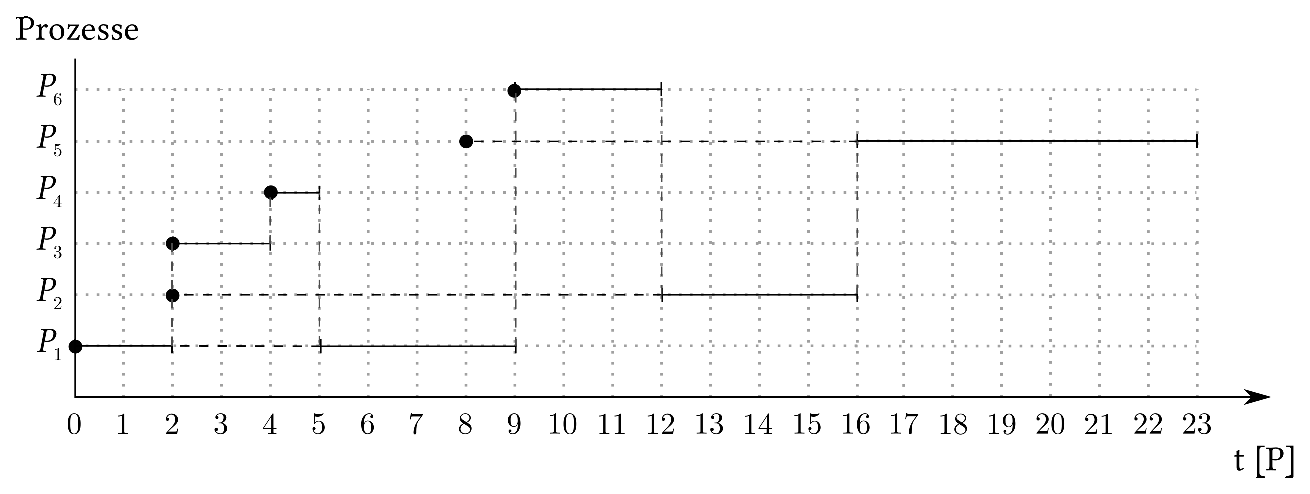
\includegraphics[width=0.9\textwidth]{23a.eps}
				\end{center}
			\item \textbf{RR} \blanko

				\begin{center}
					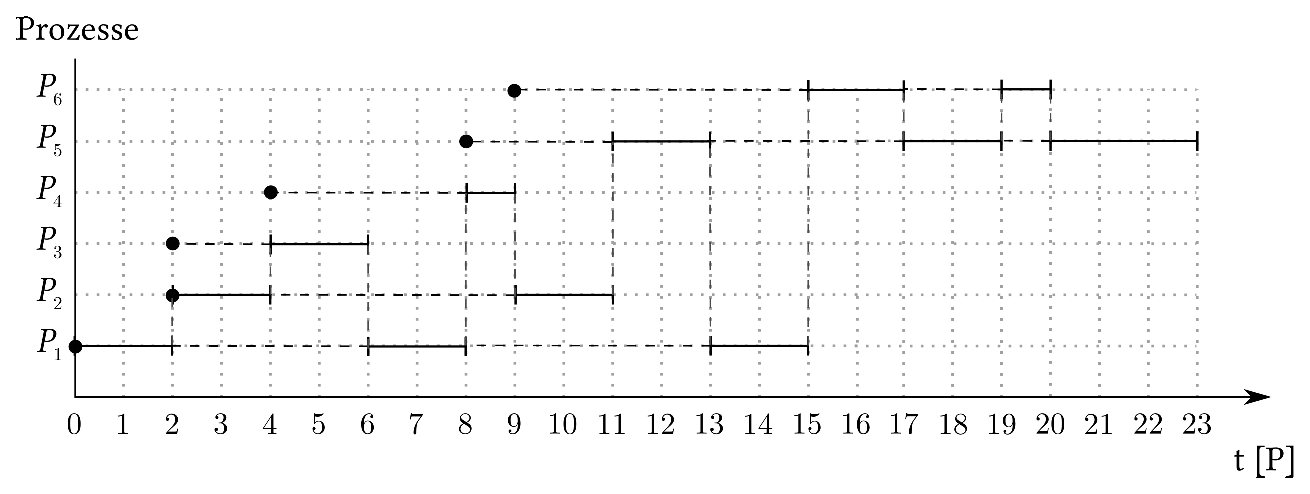
\includegraphics[width=0.9\textwidth]{23b.eps}
				\end{center}
			\pagebreak
			\item \textbf{SRPT}
				\vspace{1em}
				\begin{center}
					\small
					\renewcommand*{\arraystretch}{1.2}
					\begin{tabular}{@{}lllllr@{}lll@{}}
						\toprule
						{\footnotesize Proz.} & {\footnotesize Ankunftz.} & {\footnotesize Bedienz.} & {\footnotesize Beendigungsz.} & {\footnotesize Verweildauer} & \multicolumn{2}{c}{\footnotesize Nom. Vwd.} & {\footnotesize Wartezeit} \\ 
						\midrule
						$P_1$ & $0$ & $6$ & $9$ & $9$ & $\nicefrac{9}{6}~$&$=1,5$ & $3$ \\
						$P_2$ & $2$ & $4$ & $16$ & $14$ & $\nicefrac{14}{4}~$&$=3,5$ & $10$ \\
						$P_3$ & $2$ & $2$ & $4$ & $2$ & $\nicefrac{2}{2}~$&$=1$ & $0$ \\
						$P_4$ & $4$ & $1$ & $5$ & $1$ & $\nicefrac{1}{1}~$&$=1$ & $0$ \\
						$P_5$ & $8$ & $7$ & $23$ & $15$ & $\nicefrac{15}{7}~$&$=2,14$ & $8$ \\
						$P_6$ & $9$ & $3$ & $12$ & $3$ & $\nicefrac{2}{3}~$&$=0,66$ & $0$ \\
						\bottomrule
					\end{tabular}
				\end{center}
				\vspace{1em}

				Mittlere Verweildauer $ = (9+14+2+1+15+3)/6 = 7,33$ \\
				Mittlere normalisierte Verweildauer $ = \left(\nicefrac{9}{6} + \nicefrac{14}{4}+\nicefrac{2}{2}+\nicefrac{1}{1}+\nicefrac{15}{7}+\nicefrac{2}{3}\right)/6 = 1,63$ \\
				Mittlere Wartezeit $ = (3+10+0+0+8+0)/6 = 3,50$ 

				\textbf{RR}
				\vspace{1em}
				\begin{center}
					\small
					\renewcommand*{\arraystretch}{1.2}
					\begin{tabular}{@{}lllllr@{}lll@{}}
						\toprule
						{\footnotesize Proz.} & {\footnotesize Ankunftz.} & {\footnotesize Bedienz.} & {\footnotesize Beendigungsz.} & {\footnotesize Verweildauer} & \multicolumn{2}{c}{\footnotesize Nom. Vwd.} & {\footnotesize Wartezeit} \\ 
						\midrule
						$P_1$ & $0$ & $6$ & $15$ & $15$ & $\nicefrac{15}{6}~$&$=2,5$ & $9$ \\
						$P_2$ & $2$ & $4$ & $11$ & $9$ & $\nicefrac{9}{4}~$&$=2,25$ & $5$ \\
						$P_3$ & $2$ & $2$ & $6$ & $4$ & $\nicefrac{4}{2}~$&$=2$ & $2$ \\
						$P_4$ & $4$ & $1$ & $9$ & $5$ & $\nicefrac{5}{1}~$&$=1$ & $4$ \\
						$P_5$ & $8$ & $7$ & $23$ & $15$ & $\nicefrac{15}{7}~$&$=2,14$ & $8$ \\
						$P_6$ & $9$ & $3$ & $20$ & $11$ & $\nicefrac{11}{3}~$&$=3,67$ & $8$ \\
						\bottomrule
					\end{tabular}
				\end{center}
				\vspace{1em}

				Mittlere Verweildauer $ = (15+9+4+5+15+11)/6 = 9,83$ \\
				Mittlere normalisierte Verweildauer $ = \left(\nicefrac{15}{6} + \nicefrac{9}{4}+\nicefrac{4}{2}+\nicefrac{5}{1}+\nicefrac{15}{7}+\nicefrac{11}{3}\right)/6 = 2,93$ \\
				Mittlere Wartezeit $ = (9+5+2+4+8+8)/6 = 6,00$ 
		\end{enumerate}
	\pagebreak
	\setcounter{enumi}{25}
	\item 
		\begin{enumerate}
			\item \blanko

				\begin{center}
					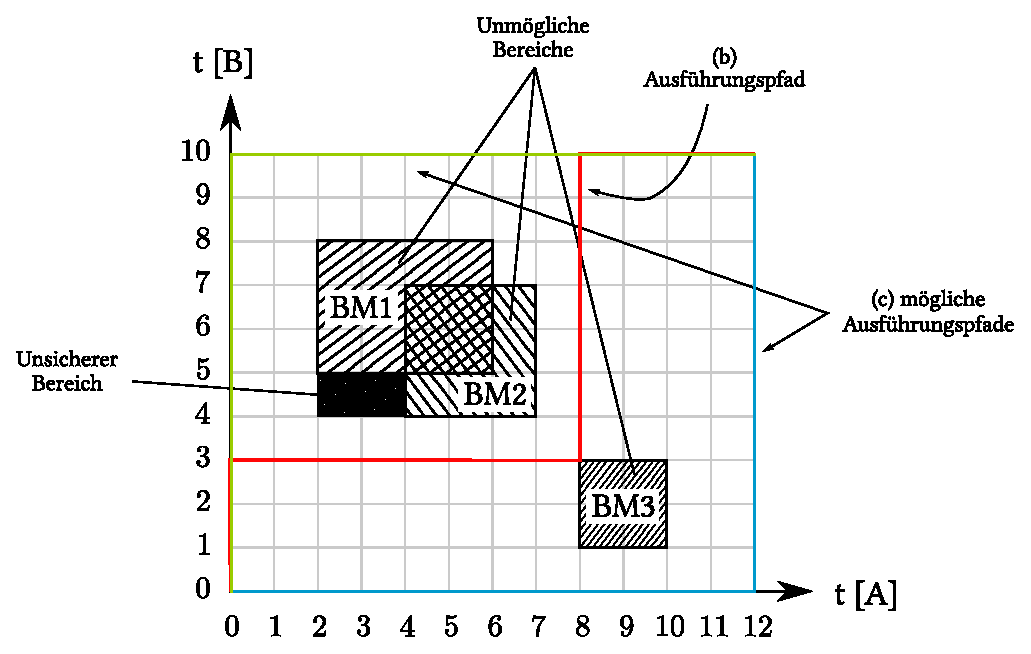
\includegraphics[width=0.9\textwidth]{26a.eps}
				\end{center}

				Es führt zu einem Deadlock, wenn der Ausführungspfad in den unsicheren Bereich kommt. Da der Ausführungspfad nur rechts und oben weitergehen kann, kommt der Graph unweigerlich in den unmöglichen Bereich.
			\item Sehen Sie bitte das obige Teil (a).
			\item Nein, es kann nicht bei nicht-präemptivem Scheduling zu einem Deadlock kommen. Bei nicht-präemptivem Scheduling sind Prozesse ohne Unterbrechungen hintereinander durchgeführt. Das heißt, dass kein Prozess muss auf einem anderem Prozess warten. Dabei kann auch kein Deadlock entstehen.

				Sehen Sie bitte das obige Teil (a) für die mögliche Abarbeitung von Prozess $A$ und $B$.
			\pagebreak
			\item Je nach dem Scheduling-Algorithm kann es zu vielen verschiendenen Abläufen führen. Man kann aber 6 prinzipiell verschiendenen Möglichkeiten bestimmen, um die Prozesse $A$ und $B$ erfolgreich terminieren zu lassen:
				\begin{itemize}
					\footnotesize
					\item $A(1) \Rightarrow A(2) \Rightarrow A'(1) \Rightarrow A'(2) \Rightarrow$ \colorbox{green!30}{$A(3) \Rightarrow A'(3)$} $\Rightarrow$  \colorbox{red!30}{$B(3) \Rightarrow B'(3)$} $\Rightarrow$ \colorbox{blue!20}{$B(2) \Rightarrow B(1) \Rightarrow$} \colorbox{blue!20}{$B'(2) \Rightarrow B'(1)$} \hfill (blauer Pfad)
					\item \colorbox{red!30}{$B(3) \Rightarrow B'(3)$} $\Rightarrow$ \colorbox{blue!20}{$B(2) \Rightarrow B(1) \Rightarrow B'(2) \Rightarrow B'(1)$} $\Rightarrow A(1) \Rightarrow A(2) \Rightarrow A'(1) \Rightarrow A'(2) \Rightarrow$  \colorbox{green!30}{$A(3) \Rightarrow A'(3)$} \hfill (grüner Pfad)
					\item \colorbox{red!30}{$B(3) \Rightarrow B'(3)$} $ \Rightarrow A(1) \Rightarrow A(2) \Rightarrow A'(1) \Rightarrow A'(2) \Rightarrow $ \colorbox{blue!20}{$B(2) \Rightarrow B(1) \Rightarrow B'(2) \Rightarrow B'(1)$} $\Rightarrow$  \colorbox{green!30}{$A(3) \Rightarrow A'(3)$}\hfill (roter Pfad)
					\item $A(1) \Rightarrow $  \colorbox{red!30}{$B(3) \Rightarrow B'(3)$} $\Rightarrow A(2) \Rightarrow A'(1) \Rightarrow A'(2) \Rightarrow$ \colorbox{blue!20}{$B(2) \Rightarrow B(1) \Rightarrow B'(2) \Rightarrow B'(1)$} $\Rightarrow$  \colorbox{green!30}{$A(3) \Rightarrow A'(3)$}
					\item \colorbox{red!30}{$B(3) \Rightarrow B'(3)$} $\Rightarrow A(1) \Rightarrow A(2) \Rightarrow A'(1) \Rightarrow A'(2) \Rightarrow$ \colorbox{blue!20}{$B(2) \Rightarrow B(1) \Rightarrow B'(2) \Rightarrow B'(1)$} $\Rightarrow$  \colorbox{green!30}{$A(3) \Rightarrow A'(3)$}
					\item $A(1) \Rightarrow $  \colorbox{red!30}{$B(3) \Rightarrow B'(3)$} $ \Rightarrow A(2) \Rightarrow A'(1) \Rightarrow A'(2) \Rightarrow$ \colorbox{blue!20}{$B(2) \Rightarrow B(1) \Rightarrow B'(2) \Rightarrow B'(1)$} $\Rightarrow$  \colorbox{green!30}{$A(3) \Rightarrow A'(3)$}
				\end{itemize}
			wobei
				\begin{center}
					\begin{tabular}{@{}lp{5cm}@{}}
						$K(i)$ & $\BM i$ wird von Prozess $k$ besitzt \\
						$K'(i)$ & Prozess $K$ gibt $\BM i$ zurück
					\end{tabular}
				\end{center}

			% Nein: Preemptives Scheduling ist nicht dterministisch. Daber kann man auch nicht vorher entscheiden, wie viele verschienedene Abläufe es gibt

			% Ja: Wenn man annimmt, dass Unterbrechungen zu diskriten Zeitpunkt geteilt
		\end{enumerate} 
	\item Sehen Sie bitte \texttt{u05-h27.txt}
\end{enumerate}